\chapter{Cloudlet Resource Management for Graceful Degradation of Service}
{\em Elasticity} is a key attribute of cloud computing.  When load
rises, new servers can be rapidly spun up.  When load subsides, idle
servers can be quiesced to save energy.  Elasticity is vital to
scalability, because it ensures acceptable response times under a wide
range of operating conditions.  To benefit, cloud services need to be
architected to easily scale out to more servers.  Such a design is
said to be ``cloud-native.''

In contrast, edge computing has limited elasticity.  As its name
implies, a cloudlet is designed for much smaller physical space and
electrical power than a cloud data center.  Hence, the sudden arrival
of an unexpected flash crowd can overwhelm a cloudlet and its wireless
network.  Since low end-to-end latency is a prime reason for edge
computing, shifting load elsewhere (e.g., the cloud) is not an
attractive solution.  {\em How do we build multi-user edge computing
  systems that preserve low latency even as load increases?}  That is
our focus.


Our approach to scalability is driven by the following observation.
Since compute resources and wireless capacity at the edge cannot be
increased on demand, the only paths to scalability are (a) to reduce
offered load, or (b) to reduce queueing delays through improved
end-to-end scheduling.  Otherwise, the mismatch between resource
availability and offered load will lead to increased queueing delays
and hence increased end-to-end latency.  Both paths require the
average burden placed by each user on the cloudlet and the wireless
channel to fall as the number of users increases.  This, in turn,
implies {\em adaptive application behavior} based on guidance received
from the cloudlet or inferred by the user's mobile device.  In the
context of Figure~\ref{fig:3tier}, scalability at the left is achieved
very differently from scalability at the right.  The relationship
between Tier-3 and Tier-2 is {\em non-workload-conserving}, while that
between Tier-1 and other tiers is workload-conserving.

With rare exceptions, reducing offered load is only possible with
application assistance.  Scalability at the edge is thus only
achievable for applications that have been designed with this goal in
mind.  We refer to applications that are specifically written for edge
computing as {\em edge-native applications.}  These applications are
deeply dependent on services that are only available at the edge (such
as low-latency offloading of compute, or real-time access to video
streams from edge-located cameras), and are written to adapt to
scalability-relevant guidance.  For example, an application at Tier-3
may be written to offload object recognition in a video frame to
Tier-2, but it may also be prepared for the return code to indicate
that a less accurate (and hence less compute-intensive) algorithm than
normal was used because Tier-2 is heavily loaded.  Alternatively,
Tier-2 or Tier-3 may determine that the wireless channel is congested;
based on this guidance, Tier-3 may reduce offered load by
preprocessing a video frame and using the result to decide whether it
is worthwhile to offload further processing of that frame to the
cloudlet.  In earlier work~\cite{Hu2015}, we have shown that even
modest computation at Tier-3 can make surprisingly good predictions
about whether a specific use of Tier-2 is likely to be worthwhile.

Edge-native applications may also use {\em cross-layer adaptation
  strategies,} by which knowledge from Tier-3 or Tier-2 is used in the
management of the wireless channel between them.  For example, an
assistive augmented reality (AR) application that verbally guides a
visually-impaired person may be competing for the wireless channel and
cloudlet resources with a group of AR gamers.  In an overload
situation, one may wish to favor the assistive application over the
gamers.  This knowledge can be used by the cloudlet operating system
to preferentially schedule the more important workload.  It can also
be used for prioritizing network traffic by using {\em fine-grain
  network slicing,} as envisioned in 5G~\cite{Contreras2018}.

Since the techniques for reducing offered workload are application-specific, we
focus on a specific class of edge-native applications to validate our ideas.
Our choice is a class of applications called {\em Wearable Cognitive Assistance}
(WCA) applications~\cite{ha2014towards}.  They are perceived to be ``killer apps'' for
edge computing because (a) they transmit large volumes of video data to the
cloudlet; (b) they have stringent end-to-end latency requirements; and (c) they
make substantial compute demands of the cloudlet, often requiring high-end GPUs.

We leverage unique characteristics of WCA applications to reduce
offered load through graceful degradation and improved resource
allocation.  Our contributions are as follows:
\begin{smitemize}
  \item{An architectural framework for WCA that enables graceful degradation under heavy load.}
  \item{An adaptation taxonomy of WCA applications, and techniques for workload reduction.}
  \item{A cloudlet resource allocation scheme based on degradation heuristics and external policies.}
  \item{A prototype implementation of the above.}
  \item{Experimental results showing up to 40\% reduction in offered load and graceful degradation in oversubscribed edge systems.}
\end{smitemize}


\section{System Model and Application Profiles}

% A complementary method to improve scalability is through judicious
% allocation of cloudlet resources among concurrent application
% services. 

Resource allocation has been well explored in many contexts
of computer systems, including operating system, networks, real-time
systems, and cloud data centers.  While these prior efforts can
provide design blueprints for cloudlet resource allocation, the
characteristics of edge-native applications emphasize unique design
challenges.

The ultra-low application latency requirements of edge-native
applications are at odds with large queues often used to maintain high
resource utilization of scarce resources.  Even buffering a small
number of requests may result in end-to-end latencies that are several
multiples of processing delays, hence exceeding acceptable latency
thresholds.  On the other hand, when using short queues, accurate
estimations of throughput, processing, and networking delay are vital
to enable efficient use of cloudlet resources.  However, sophisticated
computer vision processing represents a highly variable computational
workload, even on a single stream. For example, as shown in
Figure~\ref{fig:lego-dag}, the processing pipeline for LEGO has many
exits, resulting in highly variable execution times.

\begin{figure}
\centering
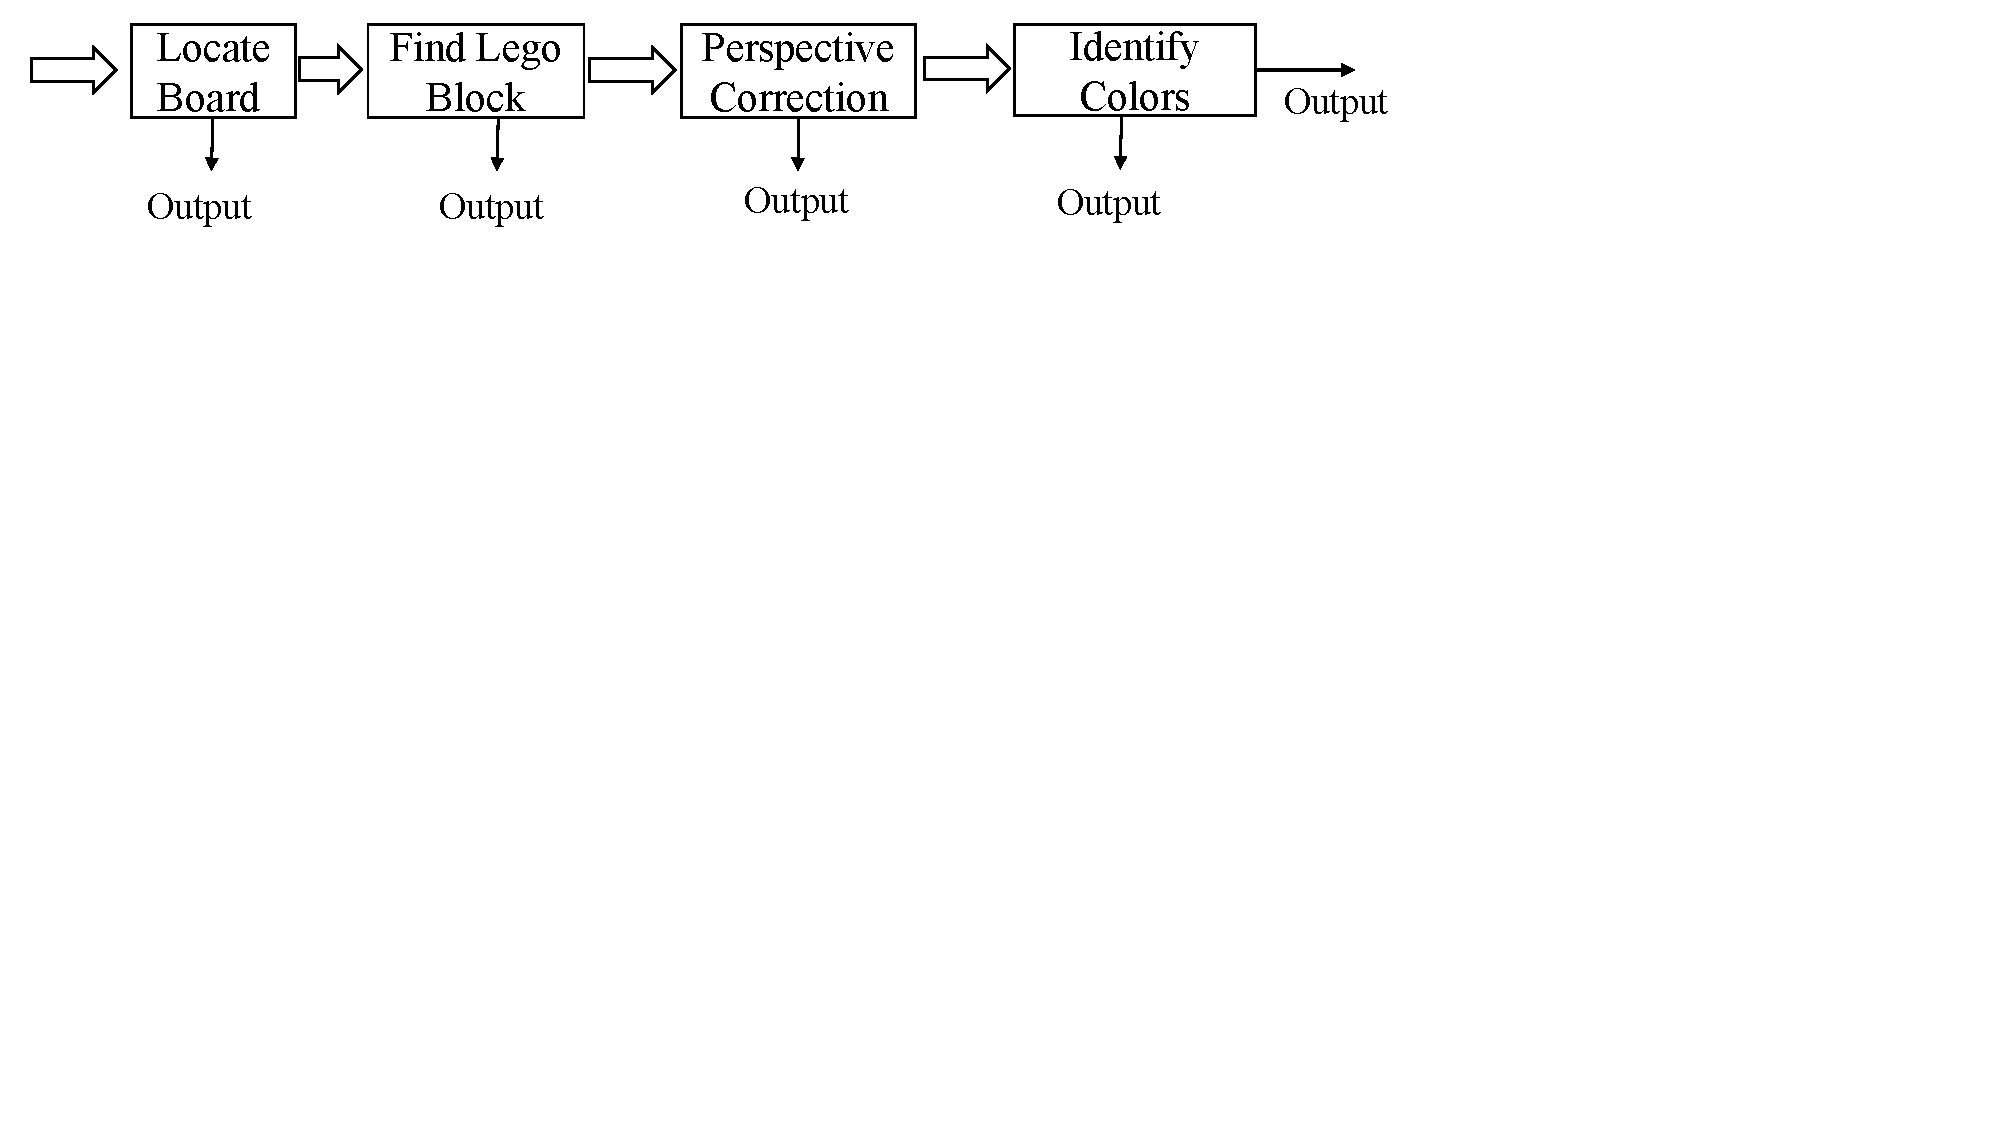
\includegraphics[width=\linewidth, trim=0em 30em 20em 0em,clip]{FIGS/fig-lego-dag.pdf}
\caption{LEGO Processing DAG}
\label{fig:lego-dag}
\end{figure}

To adequately provision resources for an application, one approach is
to leave the burden to developers, asking them to specify and reserve
a static amount of cores and memories needed for the service. However,
this method is known to be highly inaccurate and typically leads to
over-reservation in data-centers. For cloudlets, which are more
resource constrained, such over-reservation will lead to even worse
under-utilization or inequitable sharing of the available resources.
Instead, we seek to create an automated resource allocation system
that leverages knowledge of the application requirements and minimizes
developer effort.  To this end, we ask developers to provide target
Quality of Service (QoS) metrics or a utility function that relates a
single, easily-quantified metric (such as latency) to the quality of
user experience.  Building on this information, we construct offline
application profiles that map multidimensional resource allocations to
application QoS metrics.  At runtime, we calculate a resource
allocation plan to maximize a system-wide metric (e.g., total utility,
fairness) specified by cloudlet owner. We choose to consider the
allocation problem per application rather than per client in order to
leverage statistical multiplexing among clients and multi-user
optimizations (e.g., cache sharing) in an application.

\begin{figure}
\centering
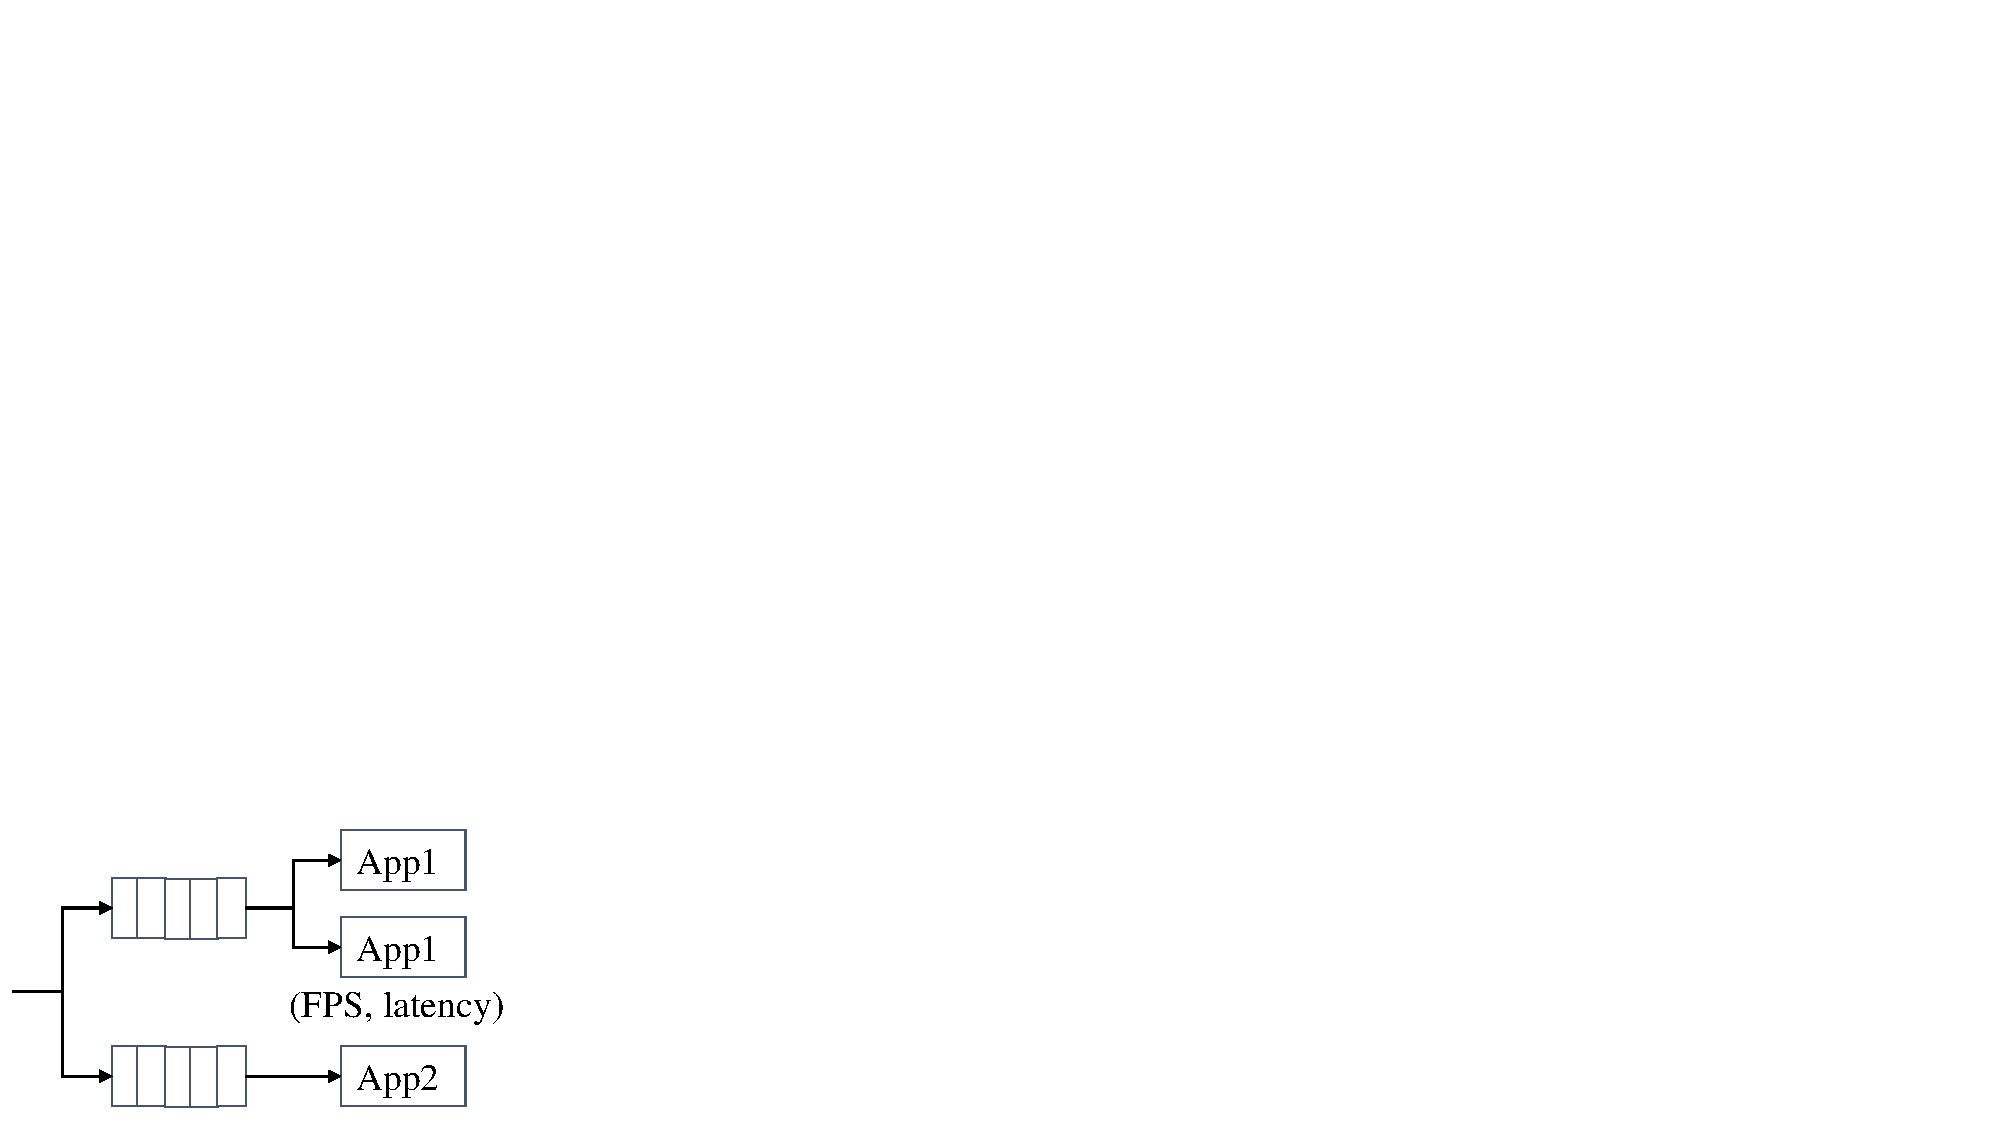
\includegraphics[width=0.5\linewidth]{FIGS/fig-allocation-system-model-cropped.pdf}
\begin{captiontext}Only request flow is shown.\end{captiontext}
\caption{Resource Allocation System Model}
\label{fig:allocation-system-model}
\vspace{-0.2in}
\end{figure}

\subsection{System Model}
Figure~\ref{fig:allocation-system-model} shows the system model we consider.
Each application is given a separate input queue. Each queue can feed one or
more application instances, which are the units of application logic that can be
replicated (e.g. a single process or several collaborative processes). Each
application instance is encapsulated in a container with controlled resources.
In this model, with adequate computational resources, clients of different
applications have minimal sharing and mainly contend for the wireless network.

We use a utility-based approach to measure and compare system-wide
performance under different allocation schemes. For WCA, the utility
of a cloudlet response depends on both the quality of response and its
QoS characteristics (e.g., end-to-end latency). The total utility of a
system is the sum of all individual utilities. A common limitation of
a utility-based approach is the difficulty of creating these
functions. One way to ease such burden is to position an application
in the taxonomy described in Section~\ref{sec:taxonomy} and borrow
from similar applications. Another way is to calculate or measure
application latency bounds, such as through literature review or
physics-based calculation as done in~\cite{chen2017empirical}.

The system-wide performance is a function of the following independent
variables. 
\begin{enumerate}[label=(\alph*)]
    \item the number of applications and the number of clients of
each application;
    \item the number of instances of each application;
    \item the resource allocation for each instance;
\end{enumerate}

Although (a) is not under our control, Gabriel is free to adapt (b) and (c).
Furthermore, to optimize system performance, it may sacrifice the performance of
certain applications in favor of others. Alternatively, it may choose not to run
certain applications.


\begin{figure}
\centering
\begin{minipage}[b]{.35\linewidth}
\centering
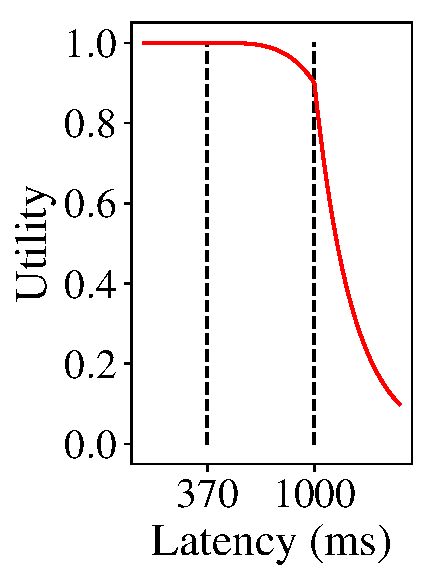
\includegraphics[width=\linewidth,trim=0em 0em 0em 0em, clip]{FIGS/fig-lat-util-face.pdf}
{(a) Utility For FACE}
\end{minipage}
\begin{minipage}[b]{.6\linewidth}
\centering
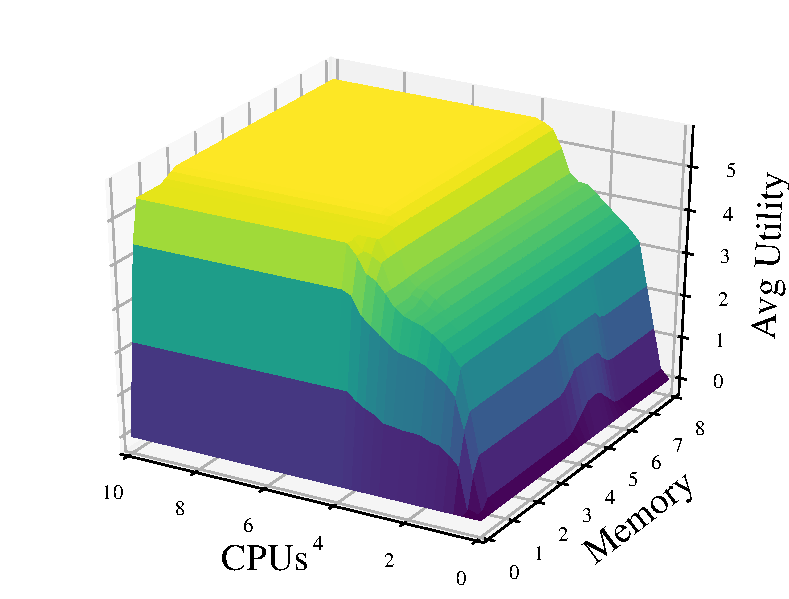
\includegraphics[width=\linewidth, trim=0em 0em 0em 0em, clip]{FIGS/fig-app-profile-face.pdf}
{(b) Profile for FACE}
\end{minipage}
\caption{FACE Application Utility and Profile}
\label{fig:face-utility-and-profile}
\end{figure}

\begin{figure}
\centering
\begin{minipage}[b]{.35\linewidth}
\centering
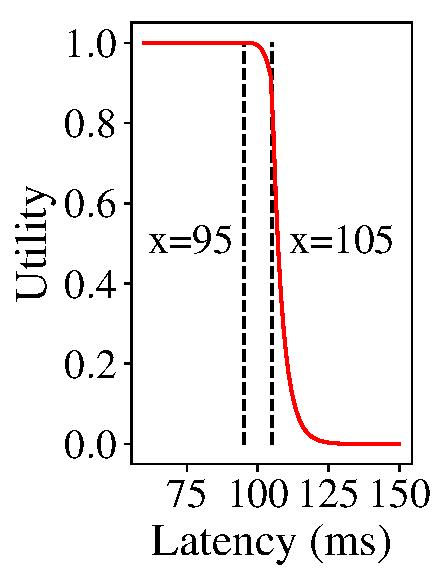
\includegraphics[width=\linewidth,trim=0em 0em 0em 0em, clip]{FIGS/fig-lat-util-pool.pdf}
{(a) Utility For POOL}
\end{minipage}
\begin{minipage}[b]{.6\linewidth}
\centering
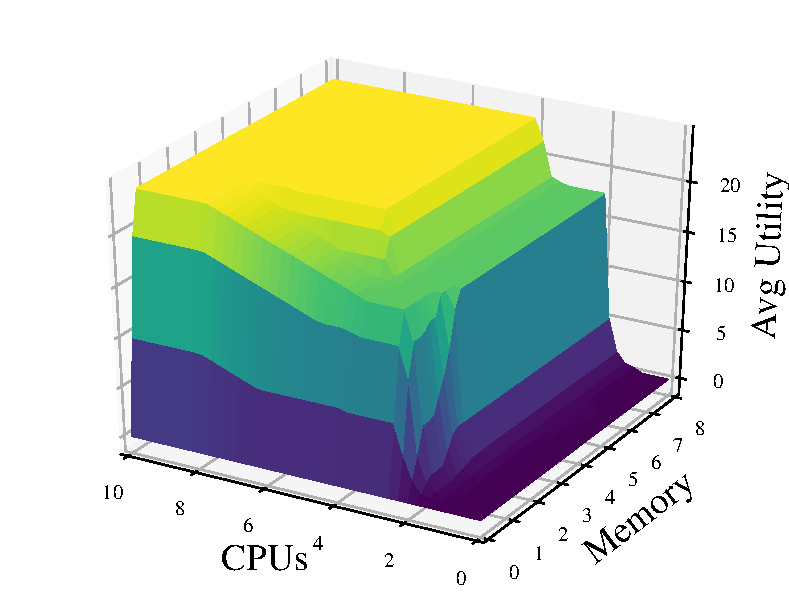
\includegraphics[width=\linewidth, trim=0em 0em 0em 0em, clip]{FIGS/fig-app-profile-pool.pdf}
{(b) Profile for POOL}
\end{minipage}
\caption{POOL Application Utility and Profile}
\label{fig:pool-utility-and-profile}
\end{figure}

\subsection{Application Utility and Profiles}

We build application profiles offline in order to estimate latency and
throughput at runtime. First, we ask developers to provide a utility
function that maps QoS metrics to application experience.
Figure~\ref{fig:face-utility-and-profile}(a) and
Figure~\ref{fig:pool-utility-and-profile}(a) show utility functions
for two applications based on latency bounds identified
by~\cite{chen2017empirical} for each request. Next, we profile an application
instance by running it under a discrete set of cpu and memory
limitations, with a large number of input requests. We record the
processing latency and throughput, and calculate the system-wide
utility per unit time. We interpolate between acquired data points of
(system utility, resources) to produce continuous functions.  Hence,
we effectively generate a multidimensional resource to utility profile
for each application.

We make a few simplifying assumptions to ensure profile generation and
allocation of resources by utility are tractable.  First, we assume utility
values across different applications are comparable. Furthermore, we assume
utility is received on a per-frame basis, with values that are normalized
between 0 and 1.  Each frame that is sent, accurately processed, and replied
within its latency bound receives 1, so a client running at 30 FPS under ideal
conditions can receive a maximum utility of 30 per second.  This clearly ignores
variable utility of processing particular frames (e.g., differences between
active and passive phases), but simplifies construction of profiles and modeling
for resource allocation; we leave the complexities of variable utility to future
work. Figure~\ref{fig:face-utility-and-profile}(b) and
Figure~\ref{fig:pool-utility-and-profile}(b) show the generated application
profiles for FACE and POOL. We see that POOL is more efficient than FACE in
using per unit resource to produce utility. If an application needs to deliver
higher utility than a single instance can, our framework will automatically
launch more instances of it on the cloudlet.

\section{Profiling-based Resource Allocation}
\label{sec: resource-allocation}

Given a workload of concurrent applications running on a cloudlet, and the
number of clients requesting service from each application, our resource
allocator determines how many instances to launch and how much resource (CPU
cores, memory, etc.) to allocate for each application instance.  We assume
queueing delays are limited by the token mechanism used in Original Gabriel,
which limits the number of outstanding requests on a per-client basis.


\subsection{Maximizing Overall System Utility}

As described earlier, for each application $a \in $ \{FACE, LEGO, PING PONG, POOL, \ldots \}, 
we construct a resource to utility mapping
$u_a: \mathbf{r} \rightarrow \mathbb{R}$ for one instance of the application on cloudlet, 
where $\mathbf{r}$ is a resource vector of allocated CPU, memory, etc. We formulate the 
following optimization problem which maximizes the system-wide total utility,
subject to a tunable maximum per-client limit:

\begin{equation}
  \begin{aligned}
  \max_{\{k_a, \mathbf{r}_a\}} \quad & \sum_a{k_a \cdot u_a(\mathbf{r}_a)} \\
  \textrm{s.t.} \quad & \sum_a k_a \cdot \mathbf{r}_a \preccurlyeq \hat{\mathbf{r}} \\
      & 0 \preccurlyeq \mathbf{r}_a  \quad \forall a \\
      & k_a \cdot u_a(\mathbf{r}_a) \le \gamma \cdot c_a \quad \forall a \\
      & k_a \in \mathbb{Z}
  \end{aligned}
  \end{equation}

In above, $c_a$ is the number of mobile clients requesting service from application $a$.
The total resource vector of the cloudlet is  $\hat{\mathbf{r}}$. 
 For each application $a$, we determine how many instances to launch --- $k_a$, and 
allocate resource vector $\mathbf{r}_a$ to each of them.
A tunable knob $\gamma$ regulates the maximum utility allotted 
per application, and serves to enforce a form of partial fairness (no application
can be given excessive utility, though some may still receive none). 
The larger $\gamma$ is, the more aggressive our scheduling algorithm
will be in maximizing global utility and
suppressing low-utility applications. 
%In our system model, the maximum $\gamma$ is 30 for
%clients at 30 FPS. 
By default, we set $\gamma=10$, which, based on our definition of
utility, roughly means resources will be allocated so 
no more than one third of frames (from a 30FPS source) 
will be processed within satisfactory latency bounds for a given
client.

Solving the above optimization problem is computationally difficult. We thus use an
iterative greedy allocation algorithm as follows.

\begin{algorithm}[H]
\SetAlgoLined
% \KwResult{Write here the result }
 Profile applications under varying resources\;
 $u_a(\mathbf{r})$: resource $\mathbf{r}$ to utility mapping for application
 $a$\;
\For{each application}{
  find the highest \emph{utility-to-resource} ratio $\frac{u_a(\mathbf{r})}{|\mathbf{r}|}$\;
}
 \While{leftover system resource}{
 Find the application with the largest \emph{utility-to-resource}
 $\frac{u_a(\mathbf{r}^*_a)}{|\mathbf{r}^*_a|}$, which has not been allocated
 resources\;
Allocate $k_a$ application instances,
each with resource $\mathbf{r}^*_a$, such that $k_a$ is the largest integer with
$k_a \cdot u_a(\mathbf{r}^*_a) \le \gamma \cdot c_a$\;
 }
 \caption{Iterative Allocation Algorithm to Maximize Overall System Utility}
\end{algorithm}

% For each application profile $u_a(\mathbf{r})$, we find the resource point that gives
% the highest $\frac{u_a(\mathbf{r})}{|\mathbf{r}|}$, i.e., \emph{utility-to-resource} ratio. 
% Denote this point as $\mathbf{r}^*_a$. We start with the application with the largest 
% $\frac{u_a(\mathbf{r}^*_a)}{|\mathbf{r}^*_a|}$. We allocate $k_a$ application instances,
% each with resource $\mathbf{r}^*_a$, such that $k_a$ is the largest integer with
% $k_a \cdot u_a(\mathbf{r}^*_a) \le \gamma \cdot c_a$. 
% If there is leftover resource, we move to the application with the next highest 
% utility-to-resource ratio and repeat the process.

In our implementation, we exploit the \texttt{cpu-shares} and
\texttt{memory-reservation} control options of Linux Docker containers. It puts
a soft limit on containers' resource utilization only when they are in
contention, but allows them to use as much left-over resource as needed.
\section{Evaluation}

We use five WCA applications, including FACE, PING PONG, LEGO, POOL, and IKEA
for evaluation~\cite{chen2017empirical,chen2018application}. These
applications are selected based on their distinct requirements and
characteristics to represent the variety of WCA apps. IKEA and LEGO assist users
step by step to assemble an IKEA lamp or a LEGO model. While their 2.7-second
loose latency bound is less stringent than other apps, the significance of their
instructions is high, as a user could not proceed without the instruction. On
the other hand, users could still continue their tasks without the instructions
from FACE, POOL, and PING PONG assistants. For POOL and PING PONG, the speed of
an instruction is paramount to its usefulness. For example, any instruction that
comes 105ms after a user action for POOL is no longer of value, because it is
too late to guide the next action.

\begin{figure}
  \centering
  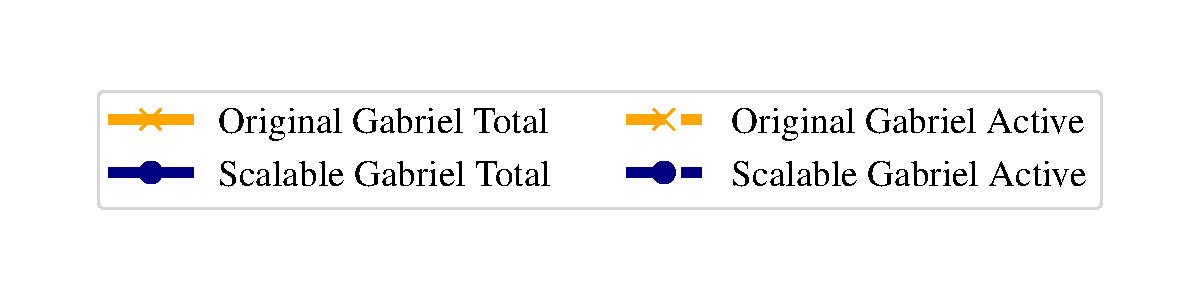
\includegraphics[width=\linewidth, trim=0em 3em 0em 3em, clip]{FIGS/fig-sec6-reduction-legend.pdf}
  \begin{minipage}[b]{0.38\linewidth}
    \centering
    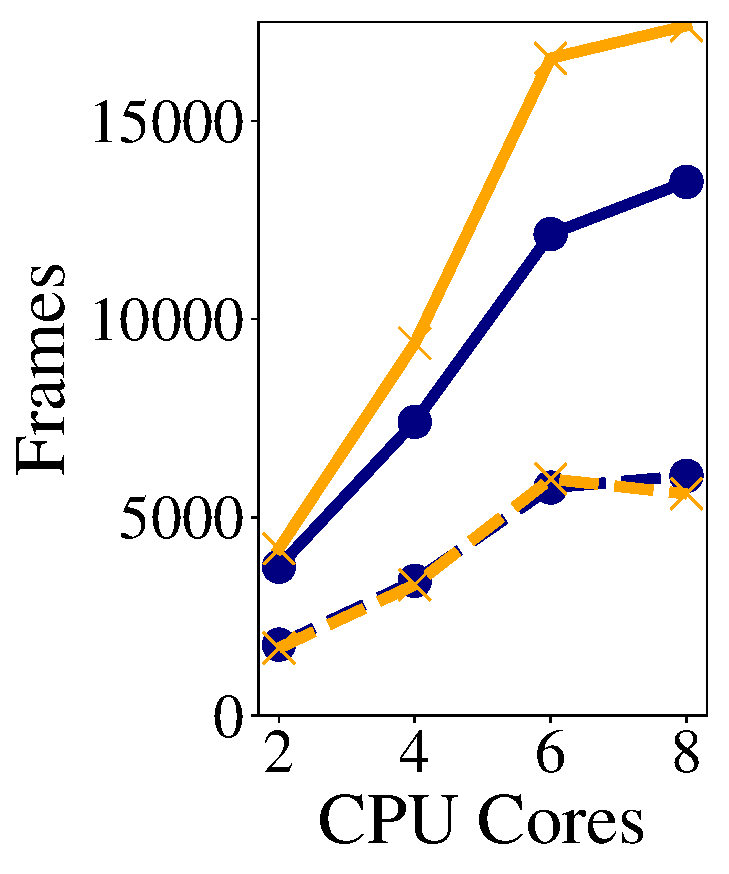
\includegraphics[height=2.5in, trim=0em 1em 0em 0em, clip]{FIGS/fig-sec6-reduction-Pingpong.pdf}\\
    {(a) PING PONG}
  \end{minipage}
  \begin{minipage}[b]{0.3\linewidth}
    \centering
    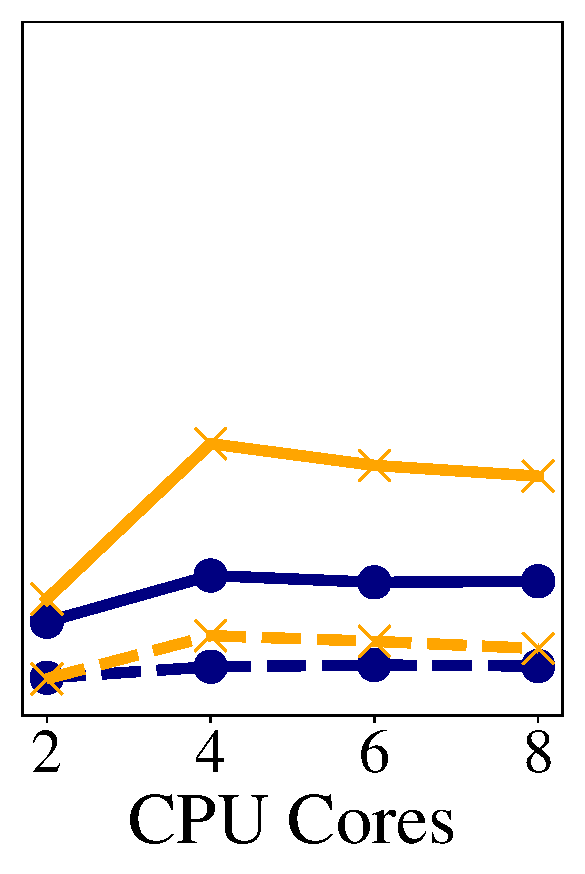
\includegraphics[height=2.5in, trim=0em 1em 0em 0em, clip]{FIGS/fig-sec6-reduction-Lego.pdf}\\
    {(b) LEGO}
  \end{minipage}
  \begin{minipage}[b]{0.3\linewidth}
    \centering
    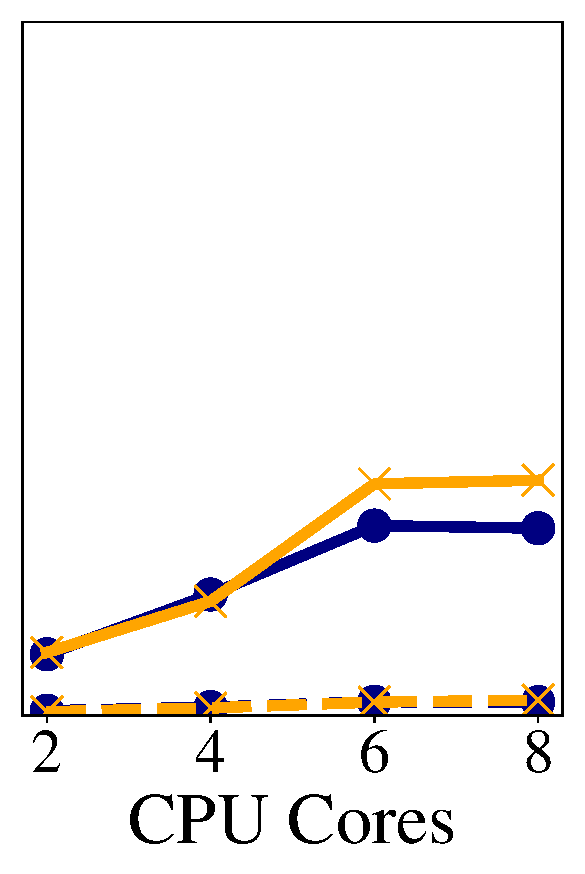
\includegraphics[height=2.5in, trim=0em 1em 0em 0em, clip]{FIGS/fig-sec6-reduction-Pool.pdf}\\
    {(c) POOL}
  \end{minipage}
  \caption{Effects of Workload Reduction}
  \label{figs:workload-reduction}
\end{figure}


\subsection{Effectiveness of Workload Reduction}

We first evaluate the effectiveness of all of the workload reduction techniques
explored in Chapter~\ref{chapter: load}. For this set of experiments, we do not
use multiple concurrent applications. Adaptation-centric cloudlet resource
allocation is not enabled for a controlled setup. We use four Nexus 6 mobile
phones as clients. They offload computation to a cloudlet over Wi-Fi links. We
run PING PONG, LEGO, and POOL applications one at a time with 2, 4, 6, and 8
cores on the edge server. We constrain the number of cores available using Linux
cgroup. Figure~\ref{figs:workload-reduction} shows the total number of frames
processed with and without workload reduction. The yellow lines for Original
Gabriel do not have workload reduction while the blue lines for Scalable Gabriel
do. The solid lines represent the total number of frames offloaded. The dashed
lines represent the number of active frames, those frames that actually contain
user state information. Note that although the offered work is greatly reduced,
the processed frames for active phases of the application have not been
affected. Thus, we confirm that we can significantly reduce cloudlet load
without affecting the critical processing needed by these applications.

\begin{table}[]
  \centering
  \begin{tabular}{|c|c||c|c|c|c|c|}
    \hline
    Exp & \multicolumn{6}{|c|}{Number of Clients}                                    \\
    \cline{2-7}
    \#  & Total                                   & FACE & LEGO & POOL & PING & IKEA \\
        &                                         &      &      &      & PONG &      \\ \hline
    1   & 15                                      & 3    & 3    & 3    & 3    & 3    \\ \hline
    2   & 20                                      & 4    & 4    & 4    & 4    & 4    \\ \hline
    3   & 23                                      & 5    & 5    & 4    & 4    & 5    \\ \hline
    4   & 25                                      & 5    & 5    & 5    & 5    & 5    \\ \hline
    5   & 27                                      & 5    & 6    & 6    & 5    & 5    \\ \hline
    6   & 30                                      & 5    & 7    & 6    & 6    & 6    \\ \hline
    7   & 32                                      & 5    & 7    & 7    & 7    & 6    \\ \hline
    8   & 40                                      & 8    & 8    & 8    & 8    & 8    \\ \hline
  \end{tabular}
  \vspace{0.1in}
  \caption{Resource Allocation Experiment Setup}
  \label{tab:alloc-exps}
\end{table}

\subsection{Effectiveness of Resource Allocation}

We next evaluate our adaptation-centric resource allocation mechanism on a
server machine with 2 Intel{\textregistered} Xeon{\textregistered} E5-2699 v3
processors, totaling 36 physical cores running at 2.3 Ghz (turbo boost disabled)
and 128 GB memory. We dedicate 8 physical cores (16 Intel{\textregistered} hyper
threads) and 16 GB memory as cloudlet resources using cgroup. We run 8
experiments with increasing numbers of clients across four concurrent
applications. The total number of clients gradually increases from 15 to 40.
Table~\ref{tab:alloc-exps} shows the breakdown of the number of clients used for
each experiment. Note that these clients are running simultaneously, resulting
in heavier and heavier contention. We generate application adapation profiles
offline using the method discussed in Section~\ref{sec: resource-allocation}. We
leverage these profiles to optimize for maximizing the total system utility.
Figure~\ref{fig:alloc-max-util} shows how the total system utility changes as we
add more clients and hence more workload. The yellow line represents the
Original Gabriel which relies on the operating system alone to divide system
resources. The blue line shows our Scalable Gabriel approach. In the beginning,
while the system is under-utilized, we see that the Original Gabriel yields
slightly higher total utility. However, as contention increases, Original
Gabriel's total utility quickly drops, eventually more than 40\%, since every
client contends for resources in an uncontrolled fashion.  All applications
suffer, but the effects of increasing latencies are vastly different among
different applications. In contrast, scalable Gabriel maintains a high level of
system-wide utility by differentially allocating resources to different
applications based on their sensitivity captured in the adaptation profiles.

\begin{figure}[h]
  \centering
  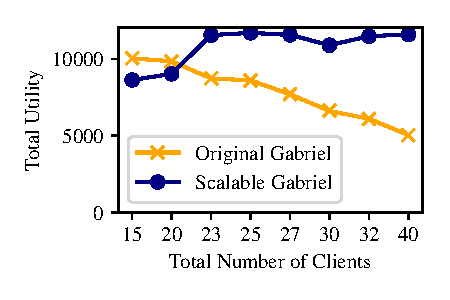
\includegraphics[width=.9\linewidth]{FIGS/fig-alloc-max-util.pdf}
  \caption{Total Utility with Increasing Contention}
  \label{fig:alloc-max-util}
\end{figure}


Figure~\ref{fig:alloc-latency} and Figure~\ref{fig:alloc-fps} provide insights
into how scalable Gabriel strikes the balance. We present both application
throughput in terms of average frames per second and latency in terms of
90\%-tile response delay. Latencies are better controlled as resources are
dedicated to applications with high utility, and more clients are kept within
their latency bounds. Of course, with higher contention, fewer frames per second
can be processed for each client. Original Gabriel degrades applications in an
undifferentiated fashion. Scalable Gabriel, in contrast, tries to maintain
higher throughput for some applications at the expense of the others, e.g. LEGO
up to 27 clients. The accuracies of application profiles influence how well
Scalable Gabriel can manage latency. Run-time resource demand could deviate
from profiles due to the differences in the request content (e.g. image
content). Profile inaccuracies result in the overshoot of POOL and IKEA
90\%-tile latencies in Figure~\ref{fig:alloc-latency}, as the profiles
underestimate their resource demand and overestimate LEGO resource demand when
the number of clients is low. When the system becomes more crowded, the
throttling of LEGO throughput reduces such an effect.

\begin{figure}[]
  \begin{center}
    
\includegraphics[width=\linewidth]{FIGS/fig-alloc-latency-legend.pdf}
    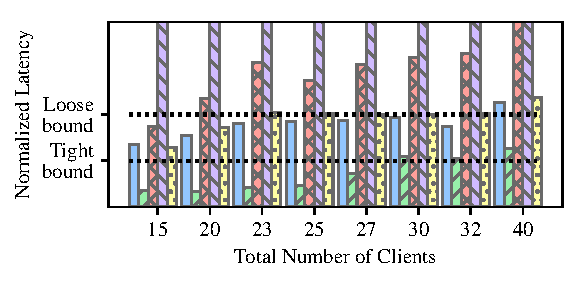
\includegraphics[width=\linewidth]{FIGS/fig-alloc-latency-baseline.pdf}
    {(a) Original Gabriel}
    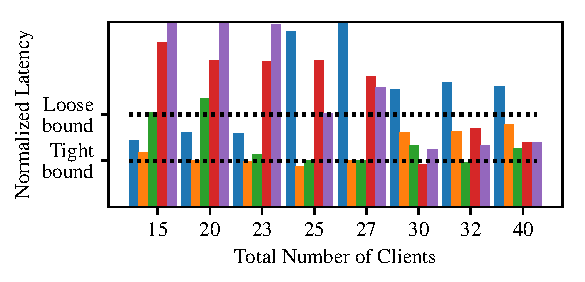
\includegraphics[width=\linewidth]{FIGS/fig-alloc-latency-cpushares.pdf}
    {(b) Scalable Gabriel}
  \end{center}
  \begin{captiontext}
    \centering
    The normalization is  by per-application tight and loose
    bounds~\cite{chen2017empirical}.

    The allocation policy is to maximize the overall system utility.
  \end{captiontext}
  \caption{Normalized 90\%-tile Response Latency}
  \label{fig:alloc-latency}
\end{figure}

\begin{figure}[]
  \begin{center}
    
\includegraphics[width=.9\linewidth]{FIGS/fig-alloc-latency-legend.pdf}
    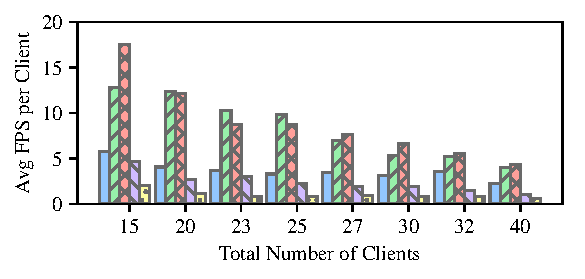
\includegraphics[width=\linewidth]{FIGS/fig-alloc-fps-baseline.pdf}
    {(a) Original Gabriel}
    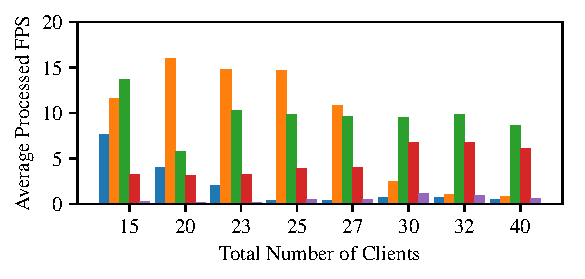
\includegraphics[width=\linewidth]{FIGS/fig-alloc-fps-cpushares.pdf}
    {(b) Scalable Gabriel}
  \end{center}
  \caption{Average Processed Frames Per Second Per Client}
  \label{fig:alloc-fps}
\end{figure}


\subsection{Effects on Guidance Latency}

We next evaluate the combined effects of workload reduction and
resource allocation in our system. We emulate many users running
multiple applications simultaneously. All users share the same
cloudlet with 8 physical cores and 16 GB memory. We conduct three experiments,
with 20 (4 clients per app), 30 (6 clients per app), and 40 (8 clients
per app) clients. Each client loops through pre-recorded video traces
with random starting points.  Figure~\ref{fig:frame-latency} and
Fig~\ref{fig:frame-fps} show per client frame latency and FPS
achieved. The first thing to notice is that concurrently utilizing
both sets of techniques does not cause conflicts. In fact, they appear
to be complementary and latencies remain in better control than using
resource allocation alone.

\begin{figure}[]
  \begin{center}
    
\includegraphics[width=\linewidth]{FIGS/fig-alloc-latency-legend.pdf}

    \begin{tabular}{c@{}c}
      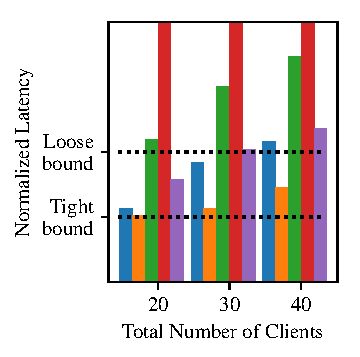
\includegraphics[width=.5\linewidth]{FIGS/fig-eval-latency-baseline.pdf}
                              & 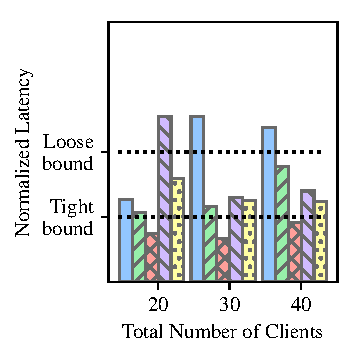
\includegraphics[width=.5\linewidth]{FIGS/fig-eval-latency-cpushares.pdf} \\
      {(a) Original  Gabriel} & {(b) Scalable Gabriel}
    \end{tabular}
  \end{center}

  \begin{captiontext}
    \centering
    The normalization is by per-application tight and loose
    bounds~\cite{chen2017empirical}.
  \end{captiontext}
  \vspace{-0.1in}
  \caption{Normalized 90\%-tile Response Latency}
  \label{fig:frame-latency}
\end{figure}

\begin{figure}[]
  \begin{center}
    % 
\includegraphics[width=\linewidth]{FIGS/fig-alloc-latency-legend.pdf}
    \begin{tabular}{c@{}c}
      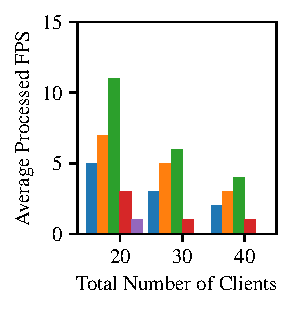
\includegraphics[width=.5\linewidth]{FIGS/fig-eval-fps-baseline.pdf}
                             & 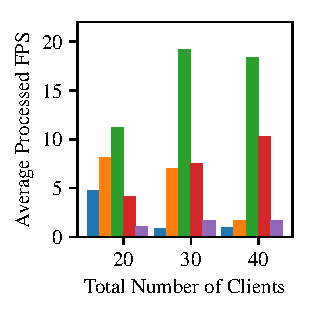
\includegraphics[width=.5\linewidth]{FIGS/fig-eval-fps-cpushares.pdf} \\
      {(a) Original Gabriel} & {(b) Scalable Gabriel}
    \end{tabular}
  \end{center}
  \caption{Processed Frames Per Second Per Application}
  \label{fig:frame-fps}
\end{figure}

\begin{figure}[]
  \begin{center}
    
\includegraphics[width=.7\linewidth]{FIGS/fig-alloc-latency-legend.pdf}
    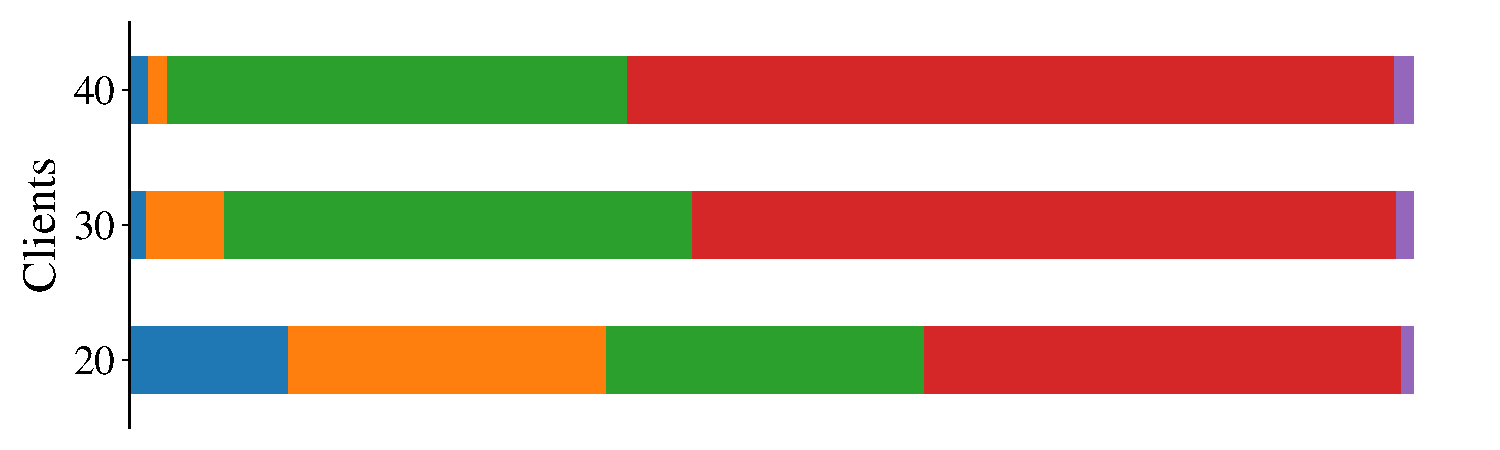
\includegraphics[width=.7\linewidth]{FIGS/fig-sec6-latency-allocation.pdf}
  \end{center}
  \vspace{-0.1in}
  \caption{Fraction of Cloudlet Processing Allocated}
  \label{figs:resource-allocated}
\end{figure}

\begin{figure}[]
  \centering
  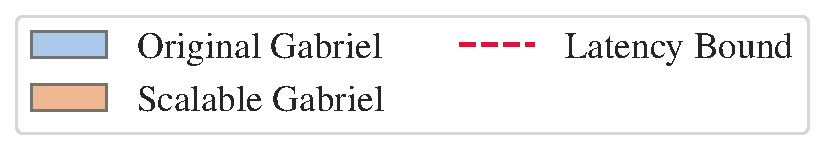
\includegraphics[width=0.5\linewidth, trim=0em 0em 0em 0em, clip]{FIGS/fig-sec6-latency-legend.pdf} \\
  \centering
  \begin{turn}{90}{\hspace{0.6in}\small (a) FACE}\end{turn}\hspace{0.2in}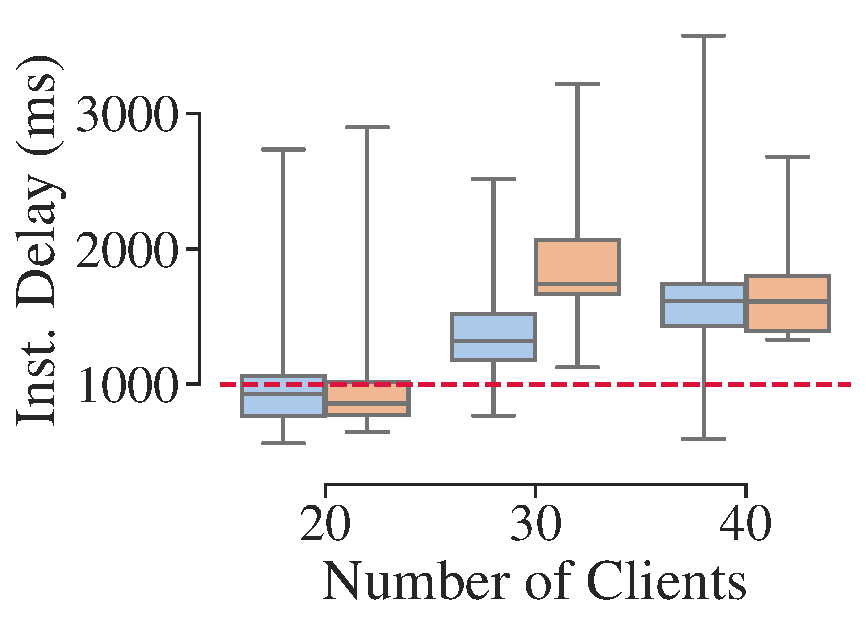
\includegraphics[width=2.5in, trim=0em 0em 0em 0em, clip]{FIGS/fig-sec6-latency-face.pdf}
  \begin{turn}{90}{\hspace{0.6in}\small (b)
      LEGO}\end{turn}\hspace{0.2in}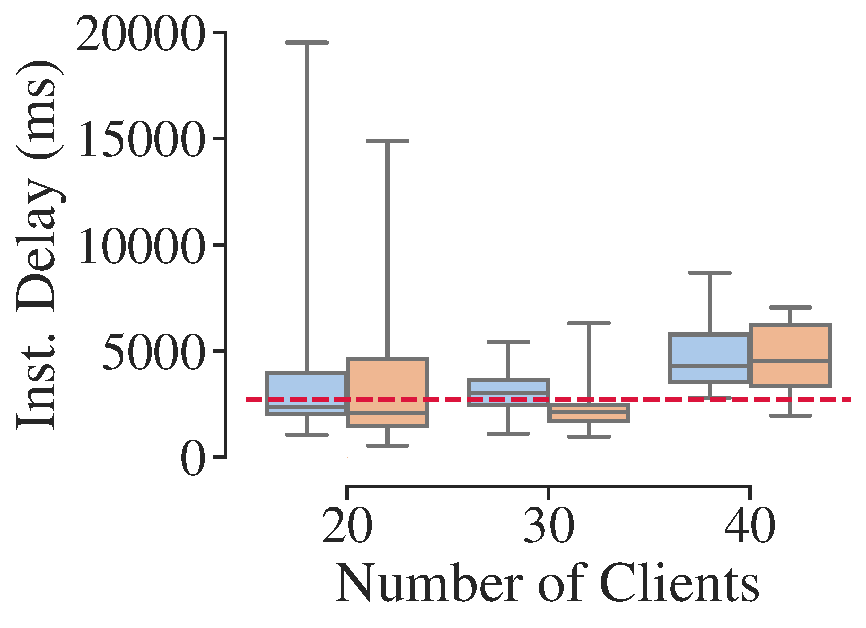
\includegraphics[width=2.5in, trim=0em 0em 0em 0em,
    clip]{FIGS/fig-sec6-latency-lego.pdf}\\[0.08in]
  \vspace{0in}
  \begin{turn}{90}{\hspace{0.6in}\small (c) PING PONG}\end{turn}\hspace{0.2in}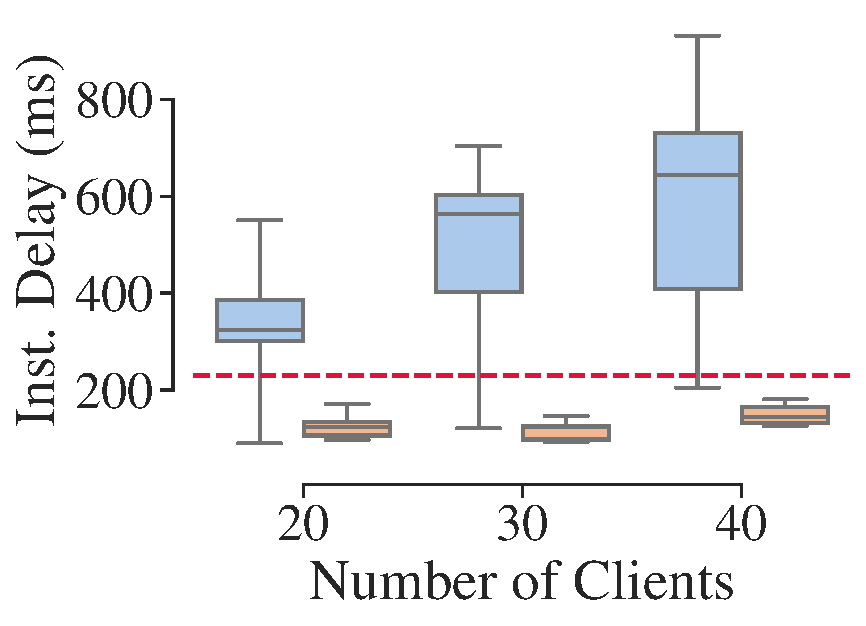
\includegraphics[width=2.5in, trim=0em 0em 0em 0em, clip]{FIGS/fig-sec6-latency-pingpong.pdf}
  \begin{turn}{90}{\hspace{0.6in}\small (d)
      POOL}\end{turn}\hspace{0.2in}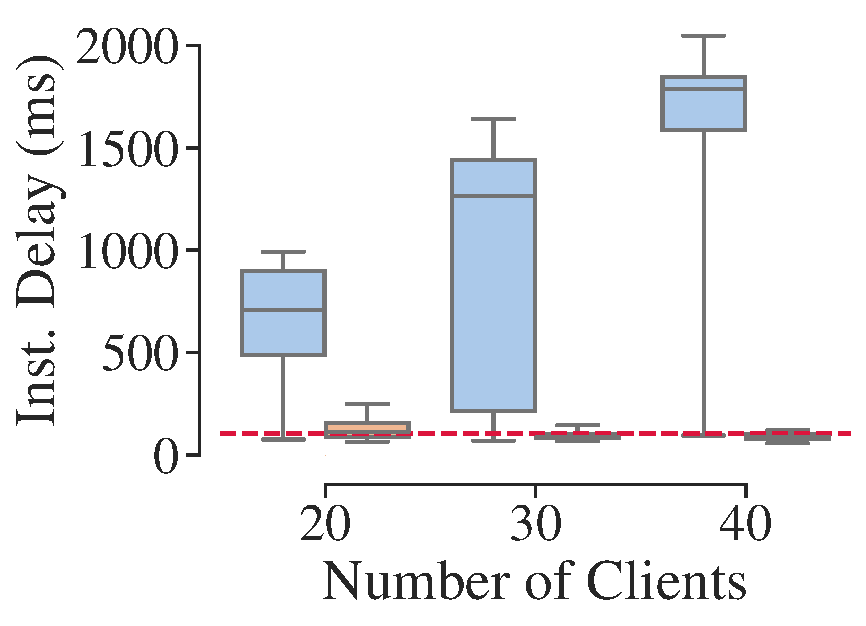
\includegraphics[width=2.5in, trim=0em 0em 0em 0em,
    clip]{FIGS/fig-sec6-latency-pool.pdf}\\[0.08in]
  \vspace{0in}
  \begin{turn}{90}{\hspace{0.6in}\small (e) IKEA}\end{turn}\hspace{0.2in}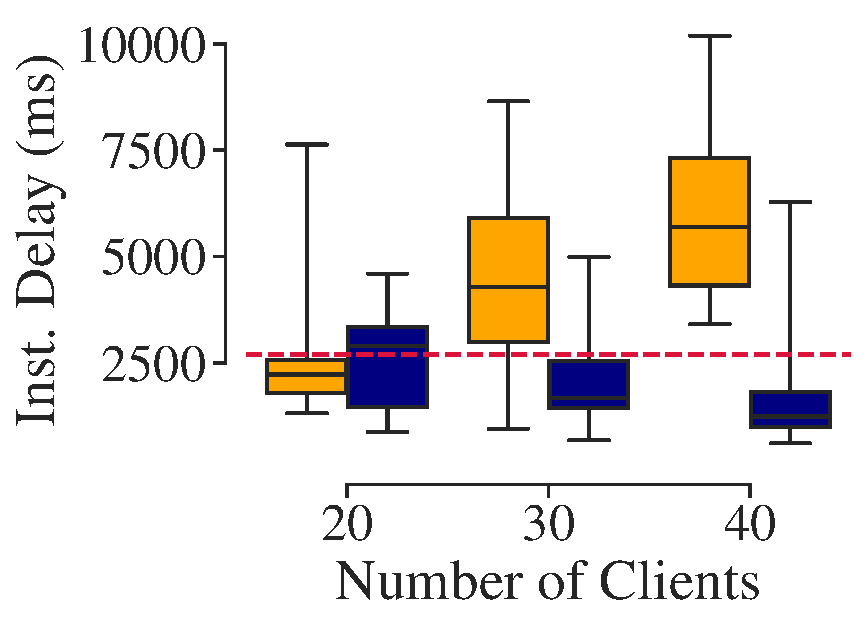
\includegraphics[width=2.5in, trim=0em 0em 0em 0em, clip]{FIGS/fig-sec6-latency-ikea.pdf}
  \caption{Guidance Latency Compared to Loose Latency Bound}
  \label{figs:inst-delay}
\end{figure}

The previous plots consider per request latencies. The ultimate goal of our work
is to maintain user experience as much as possible and degrade it gracefully
when overloaded. For WCA applications, the key measure of user experience is
guidance latency, the time between the occurrence of an event and the delivery
of corresponding guidance. Note that guidance latency is different than per
request latency, as a guidance may need not one but several frames to recognize
a user state. Figure~\ref{figs:inst-delay} shows boxplots of per-application
guidance latency for the concurrent application experiments above. The red
dotted line denotes the application-required loose bound. It is clear that our
methods control latency significantly better than the baseline. Scalable Gabriel
is able to serve at least 3x number of clients when moderately loaded while
continuing to serve more than half of the clients when severely loaded. In these
experiments, the utility is maximized at the expense of the FACE application,
which provides the least utility per resource consumed. At the highest number of
clients, scalable Gabriel sacrifices the LEGO application to maintain the
quality of service for PINGPONG and POOL. This differentiated allocation is
reflected in Figure~\ref{figs:resource-allocated}. In contrast, with original
Gabriel, none of the applications are able to regularly meet deadlines.
\section{R\lc{elated} W\lc{ork}}
\label{sec: resource-management-related}

Deadline-based scheduling algorithms and mechanisms have been studied
extensively in the literature. Many work~\cite{tokuda1990real, kao1993deadline,
    stankovic2012deadline, steiger2004operating} exist in the context of real-time
systems. Some use utility functions for scheduling tasks with soft
deadlines~\cite{ravindran2005recent, li2004utility}. While we draw
inspiration from these systems, our resource allocation focuses on application
adaptation characteristics in addition to meeting latency requirements.
Many mobile systems leverage application adaptation. Notably,
Odyssey~\cite{Noble1997} and extensions~\cite{Flinn1999} proposed upcall-based
collaboration between a mobile's operating system and its applications to adapt
to variable wireless connectivity and limited battery. Such adaption was purely
reactive by the mobile device; in our context, adaptation for a collection of
devices can be centrally managed by their cloudlet, with failover to reactive
methods as needed. Exploration of tradeoffs between application fidelity and
resource demand led to the concept of {\em multi-fidelity
        applications}~\cite{Satya1999}; such concepts are relevant to our work, but the
critical computing resources in our setting are those of the cloudlet rather
than the mobile device. More recently,
~\cite{boutin2014apollo,yao2014haste,verma2015large,ousterhout2013sparroW,delimitrou2014quasar,schwarzkopf2013omega}
study cluster scheduling in data-center context. These systems target a diverse
range of workload, take resource reservation demands, and focus on the
scalability of scheduling. In contrast, our resource allocation scheme focuses
on edge-native applications, in particular, wearable cognitive assistance, and
profile their characteristics for better outcomes in oversubscribed edge
scenarios. Closely related, dynamic resource management in the cloud for video
analytics have been explored by~\cite{sembiring2013dynamic, fu2015drs,
    kaseb2015cloud}. Some also leverage profile-based adaptation for more efficient
video analytics resource management~\cite{zhang2017live, hung2018videoedge,
    jiang2018chameleon}. However, most of these systems focus on throughput-oriented
analytics application on large clusters. In contrast, we target interactive
performance on relatively small edge deployments.



\section{C\lc{onclusion} \lc{and} F\lc{uture} W\lc{ork}}
\label{sec:conclusion}


More than a decade ago, the emergence of cloud computing led to the
realization that applications had to be written in a certain way to
take full advantage of elasticity of the cloud.  This led to the
concept of ``cloud-native applications'' whose scale-out capabilities
are well matched to the cloud, as well as tools and techniques to
easily create such applications.

The emergence of edge computing leads to another inflection point in
application design.  In particular, it leads to ``edge-native
applications'' that are deeply dependent on attributes such as low
latency or bandwidth scalability that can only be obtained at the edge.
However, as this paper has shown, edge-native applications have to be 
written in a way that is very different from cloud-native applications
if they are to be scalable.

The is the first work to show that cloud-native implementation
strategies that focus primarily on dynamic scale-out are unlikely to
be effective for scalability in edge computing.  Instead, edge-native
applications need to adapt their network and cloudlet resource demand
to system load.  As the total number of Tier-3 devices associated with
a cloudlet increases, the per-device network and cloudlet load has to
decrease.  This is a fundamental difference between cloud-native and
edge-native approaches to scalability. 

In this paper, we explore client workload reduction and server resource
allocation to manage application quality of service in the face of contention
for cloudlet resources. We demonstrate that our system is able to ensure that in
overloaded situations, a subset of users are still served with good quality of
service rather than equally sharing resources and missing latency
requirements for all.

This work serves as an initial step towards practical resource management for
edge-native applications. There are many potential directions to explore further
in this space. We have alluded to some of these earlier in the paper. One
example we briefly mentioned is dynamic partitioning of work between Tier-3 and
Tier-2 to further reduce offered load on cloudlets.  In addition, other resource
allocation policies, especially fairness-centered policies, such as max-min
fairness and static priority can be explored when optimizing overall system
performance. These fairness-focused policies could also be used to address
aggressive users, which are not considered in this paper.  While we have shown
offline profiling is effective for predicting demand and utility for WCA
applications, for a broader range of edge-native applications, with ever more
aggressive and variable offload management, online estimation may prove to be
necessary. Another area worth exploring is the particular set of control and
coordination mechanisms to allow cloudlets to manage client offered load
directly. Finally, the implementation to date only contains allocation of
resources but allows the cloudlet operating system to arbitrarily schedule
application processes.  Whether fine-grained control of application scheduling
on cloudlets can help scale services remains an open question.


% \section{Evaluation of Cloudlet Resource Management}
% \section{End-to-End Evaluation of Resource Management}